\documentclass[11pt]{article}


\marginparwidth 0.5in 
\oddsidemargin 0.25in 
\evensidemargin 0.25in 
\marginparsep 0.25in
\topmargin 0.25in 
\textwidth 6in \textheight 8 in

\usepackage{multirow}
\usepackage{tabularx}
\usepackage{longtable}
\usepackage{graphicx}
\usepackage{float}
\usepackage{natbib}


\begin{document}
\author{Ankit Sharma - MT16121}
\title{ACB-Assignment 5 and 6}
\maketitle

\section{Problem 1-RNA Sequencing\cite{doi:10.1093/nar/gkq041}}

\subsection{Task 1 - Selection of RNA based study}
Command for downloading SRA files:\\
\textbf{wget - c ftp\_path\_to\_the\_sra\_file}

Command for obtaining the corresponding fastq files:\\
\textbf{fastq-dump filename.sra}

\subsection{Task 2 - Perform quality check and generate sam files}
Command for performing quality check:\\
\textbf{fastqc filename.fastq} 

Command for downloading the index file:\\
\textbf{curl -O ftp\_path\_to\_the\_index\_file.fa.gz}

Command for unzipping the downloaded file:\\
\textbf{gunzip index\_file\_name.fa.gz}

Command for building the index file:\\
\textbf{bowtie2-build index\_file\_name.fa index\_file\_name}

Command for generating SAM file:\\
\textbf{bowtie2 -x index\_file\_name -U fastq\_file\_name -S output\_file\_name}

\subsection{Task 3 - Get raw data count using bam files and gtf file}

Command for obtaining raw counts:\\
\textbf{htseq-count output\_file\_name gtf\_file\_name}

\subsection{Task 4 - Perform normalization and clustering techniques}
Geometric mean normalization was performed followed by KMeans clustering. Data was visualized after dimensionality reduction using PCA and was visualized using matplotlib. Details of the clustering algorithm as well as PCA is present in the next section of 'Clustering on single cell data'. 100 \% accuracy was obtained for KMeans clustering. The screen shot and plots are as follows:

\begin{figure}[H]
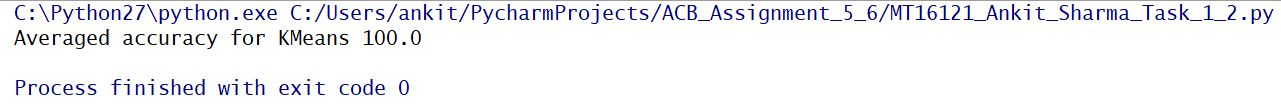
\includegraphics[width=12cm]{Accuracy_Task_1.JPG}
\end{figure}

\begin{figure}[H]
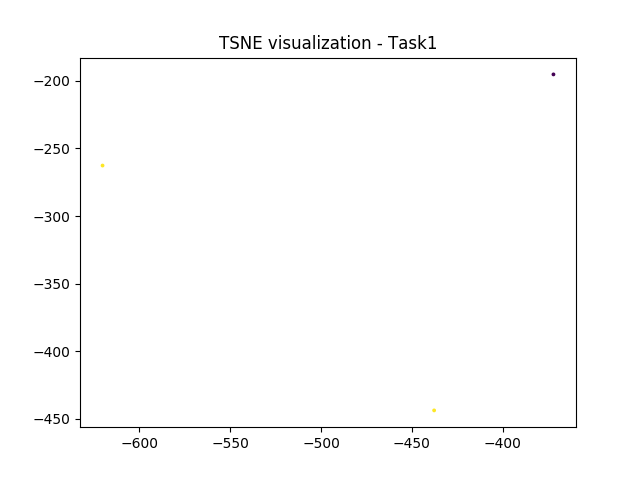
\includegraphics[width=10cm]{Task_1_TSNE_Visualization.png}
\end{figure}

\begin{figure}[H]
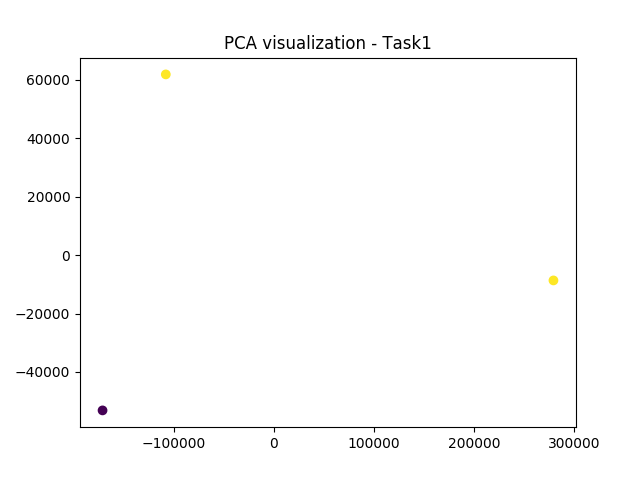
\includegraphics[width=10cm]{Task_1_PCA_Visualization.png}
\end{figure}

\subsection{Task 5 - Significance of the biological data}
The following SRA files for homosapiens were used:\\
1. SRR015164.sra\\
2. SRR015165.sra\\
3. SRR015166.sra\\
The study of which these samples are a part of is 'Prediction of alternative isoforms from exon expression levels in RNA-Seq experiments'. Using these data files, methods were developed to predict alternate isoforms derived solely from exon expression levels in RNA-seq data. These three data points were clustered in two on the basis of literature. This dataset thereby aids alternative isoform analysis.


\section{Problem 2-Clustering on single cell data\cite{10.1371/journal.pbio.1000480}}

This problem was coded using python 2.7 and the code is shared along with this report.

\subsection{Task 1 - Normalization and log transform}
The single cell study downloaded from recount database was 'Polymorphic cis- and trans-regulation of human gene expression'. This study dealt with 1,000 human genes with the motive to identify cis and trans acting polymorphic regulators. Two files were downloaded, 'cheung\_count\_table.txt' and 'cheung\_phenodata.txt'. The first file consisted of a matrix in which rows represented genes and columns represented samples. The second file consisted of phenotype information for each and every sample which was used as the ground truth. The text files were read and a corresponding list of lists was created in python. The normalization technique used for this task was 'Geometric mean normalization'. To normalize data using this technique, each and every read count is divided by the geometric mean of the gene corresponding to that read count across all samples. This normalized matrix then underwent log transformation, in which log(1 + read\_count) with base 2 was computed for every read count. This log normalized matrix was then written to 'log\_norm.csv'.

\subsection{Task 2 - Clustering}
The three clustering techniques used were Spectral clustering, Agglomerative clustering and K Means clustering. The data was split into training and testing with the test data size as 30\%. As the clustering depends upon the random split of data, therefore to ensure robust results, average accuracy was computed for 100 runs. Explanation about the clustering techniques used are as:

\subsubsection{Spectral Clustering}
Spectral clustering makes use of the eigenvalues of the Laplacian matrix to perform dimensionality reduction to a lesser number of dimensions. Once, the dimensions get reduced, the points are clustered on the basis of the number of cluster centers that are provided as the input. Sklearn's "SpectralClustering" class was used to implement this kind of clustering with the number of clusters equal to 2. Predictions were obtained for the test input data and the predicted clusters were then compared with the ground truth for accuracy. An accuracy of 41.53 \% was obtained using this technique. This technique was chosen as laplacian aims at capturing the neighbourhood of a data point which is an important aspect when we go for clustering.

\subsubsection{Agglomerative Clustering}
Agglomerative clustering is a special type of hierarchical clustering technique that makes use of the botton up approach. In this each data point begins in its own cluster and gets merged as we move up in the hierarchy. Sklearn's "AgglomerativeClustering" class was used for implementation with number of clusters equal to 2. The averaged out accuracy was 46.15\%. Hierarchical clustering is best suited for genomic data that was the reason why I went for this technique.

\subsubsection{KMeans clustering}
This clustering technique aims to divide the data set into k clusters in which each data point belongs to a cluster with the nearest mean. The averaged out accuracy for KMeans clustering was 69.23\%. Although this technique gave the highest accuracy but was the slowest of all. The algorithm took a lot of time to converge with respect to other two methods.

\subsection{Task 3 - t-SNE and PCA}
\subsubsection{TSNE}
TSNE stands for t-Distributed Stochastic Neighbor Embedding. This is a dimensionality reduction technique that is used for reducing very high number of dimensions to a lower number which can then be used for visualization. Sklearn's TSNE package was used for its implementation and then sklearn's matplotlib was used to visualize it. The plot is available in the following subsection. Data points are coloured on the basis of their clusters from the ground truth.

\subsubsection{PCA}
PCA stands for Principal Component Analysis. It is a statistical technique that uses orthogonal transformation to reduce dimensions. The first principal component has the highest variance, the second one has the second highest variance and so on. It is commonly used to visualize genetic distances among populations and that is the reason we have used it here. Sklearn's PCA class was used for the implementation followed by the used of matplotlib.

\subsubsection{Accuracy and Plots}

The screen shot for the accuracy is as follows:
\begin{figure}[h]
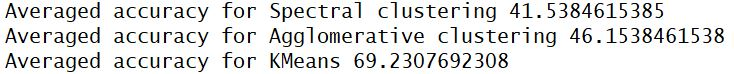
\includegraphics[width=12cm]{Accuracy.JPG}
\end{figure}

The plot for TSNE visualization is as follows:
\begin{figure}[H]
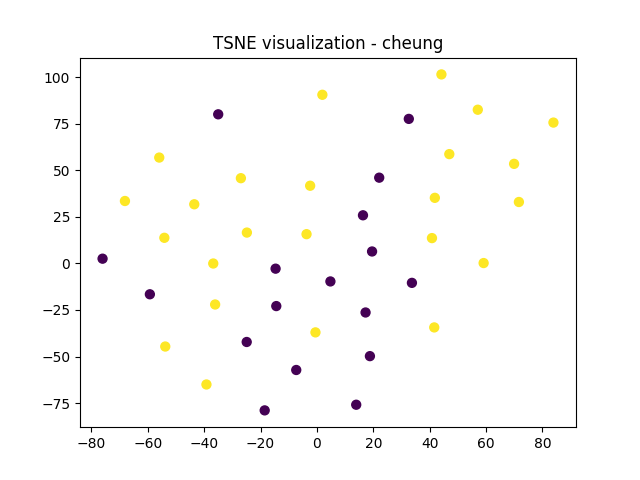
\includegraphics[width=10cm]{TSNE_Visualization.png}
\end{figure}

The plot for PCA visualization is as follows:
\begin{figure}[H]
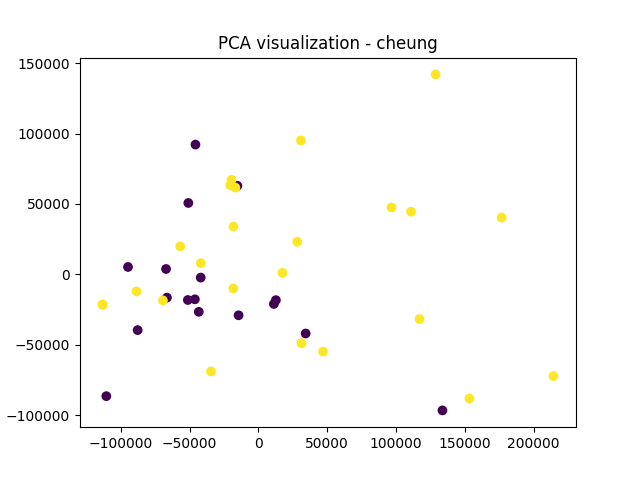
\includegraphics[width=10cm]{PCA_Visualization.png}
\end{figure}

\subsection{Task 4 - Biological significance of the data}
The data used in this study contains gene expression levels for various samples. There exists a direct correlation between gene expression levels and the phenotype exhibited but this has not been validated molecularly. Also, due to the complex nature of humans as biological systems, there exists a great amount of variability in the gene expression levels. This variation causes the human body to exhibit variations like differences in disease susceptibility etc. Thus, the biological data encountered in this study aims to bridge the gap in between genotype and phenotype. 

\section{Deliverables}
All the code files, plots and scripts are checked in to BitBucket by the name of hw5\_6\_mt16121 and the repository is shared with ayalurarvind@gmail.com.

\bibliographystyle{plain}
\bibliography{references}

\end{document}
